\documentclass[11pt,en]{elegantpaper}
\usepackage{graphicx}
\usepackage{float}
\title{The Classification and Prediction of Diabetes Dataset}
\author{Wangzhihui Mei 2019124044 \\ Hongyi Huang 201912xxxx \\ Zijia He 201912xxxx \\ Chang Xu 201912xxxx}
\institute{CCNU-UOW JI}

\begin{document}

\maketitle



\section{Introduction}
The data set we used was collected by the 
National Institute of Diabetes and Digestive and Kidney Diseases 
from a group of women and Pima Indian descendants at least 21 years old. The goal is to use patient information to predict whether a patient has diabetes.
There are 8 features:\\
\begin{itemize}
    \item Number of times pregnant
    \item Plasma glucose concentration a 2 hours in an oral glucose tolerance test
    \item Diastolic blood pressure (mm Hg)
    \item 2-Hour serum insulin (mu U/ml)
    \item Triceps skin fold thickness (mm)
    \item Body mass index (weight in kg/$(height in m)^2$)
    \item Diabetes pedigree function
    \item Age (years)
\end{itemize}

And 1 label (response variable). These data are collected from actual patients and represent a task, 
usually performed by a human doctor, with the purpose of identifying the patients most likely to have
diabetes in order to propose preventive measures. \\
Next, we conducted some comparative studies on these data, we can get a table:\\
\begin{figure}[H]
    \centering
    
\includegraphics[scale=0.6]{figure/1.PNG}  
\end{figure}

\begin{figure}[H]
    \centering
    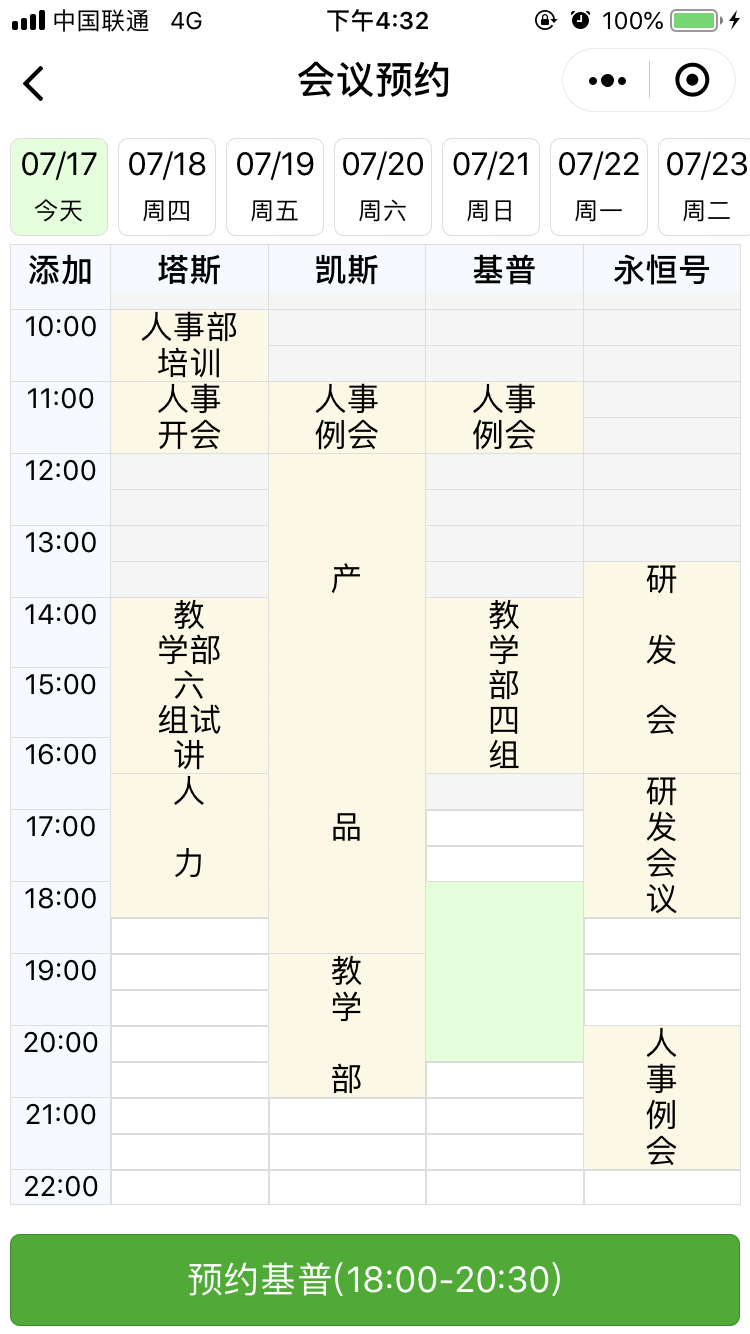
\includegraphics[scale=0.6]{figure/2.PNG}  
\end{figure}

\section{Deep Learning effectiveness}


\section{Methodologies}


\subsection{Comparison}


\section{Conclusion}


%\bibliography{wpref}

\end{document}
